\chapter{Experiments}

    The purpose of this chapter is to overview the experiments phase of the project, that contains the work done to deploy and measure how the system performs in a simulated scenario.
    Whereas the developed unit tests in the implementation stage aim to verify the correct functionality of separate units of code pertaining to the system, the execution of the entire system as a whole to serve a set of hypothetical use cases can help achieve a better grasp on how correct system functionality between all the tested units.
    Adjacent to the goal of testing the system in deployed scenarios, the experiments phase also aims to embed in the simulated environment a list of application scenarios that could leverage the \gls{alto} system to its advantage, and subsequently observe and measure if and how the \gls{alto} server can help the client with its network resources that guide the client in taking application decisions that aim for a win-win scenario between the overlay and underlay.
    As comparison, other known application-network interaction strategies will also be observed and their results measured as a means to compare their impact in comparison to one that utilizes the implemented system.
    Findings on existing application-layer traffic optimization interactions and the proposal of the \gls{alto} protocol made on section \ref{sec:state-of-art}, together with the specified system extensions on \ref{sec:specification} leads one to believe that a theoretical mutually beneficial scenario exists in an \gls{alto} approach that cannot exist with more asymmetrical means of interaction.
    This chapter, however, puts those theoretical scenarios into a practical environment that could be replicated by those reading this work, and exposing the created scenarios and collected data can corroborate the theoretical conclusions, as well as leaving an opportunity for future discussion on how the system behaved, including its performance, its success in aiding clients, other existing client options that could be a better route, system shortcomings, etc.
    This discussion benefits the \gls{alto} project and can give more maturity to the system as it was put through a simulated deployment against other common strategies.

    The first section displays the chosen technologies for tasks pertaining to the experiments.
    The next section focuses on the required steps taken to setup the testing environment.
    This includes the design and deployment of a network topology in a simulation, the creation of mock applications to serve as clients for the system, and the design and deployment of application and network status measurement tools.
    The following section individually overviews the devised scenarios to test in the simulation, and with it experiment specifics such as the initial problem, what strategies will be tested to solve it, how many runs will be made per strategy, and what metrics will be measured.
    Finished the experiments, the following section will display the obtained results that were collected in the simulated environment, and the section after that will discuss these results and how they fare with the theoretical findings.

\section{Technologies Used}

    The \gls{core} \cite{core} was used as a network simulator and represents the backbone of the experiments as a whole as it will serve as the background for the running scenarios.
    This tool allows for the creation and emulation of network environments, and with it are included the abilities to construct network topologies and manipulate properties of the member nodes, which can include network routers, switches, and host machines, that will all be used for the designed experiment scenarios.
    Additionally, link connection properties can themselves be customized, as parameters like max bandwidth, packet loss percentage, or packet delay can be meticulously customized, and in fact will be in the upcoming scenarios as a means to simulate a given circumstance that may occur in a realistic environment, such as link inefficiency that results from peak traffic hours.
    Another property that was of great importance for its selection on this work is that, on top of the virtual network environment, arbitrary code can be run on behalf of a given entity and can be addressed to another, acting as if it were an actual network.
    This will be leveraged to run software pre-packaged in the emulator, such as routing protocols that are essential for the correct expected behavior of a simulated network, but also to schedule software execution that was developed for this work, which includes the \gls{alto} server, network state providers - e.g., probing daemons and application feedback collectors - and system clients for the \gls{p2p} and \gls{http} mock applications that will be devised to play out a particular experiment scenario, and which will have embedded into it an \gls{alto} client to interface with the server for council.
    As the simulation tool runs on Linux and builds a simulated network that behaves very much like a real one, well known real-application tools can be used on top of it in other needed areas, including the deployment and measuring phases, which gives plenty of flexibility on tool selection.

    Python \cite{python} will be utilized to implement all simple software prototypes whose purpose is uniquely to test the application in a real scenario. \cite{python}
    This includes the \gls{p2p} file-transfer applications, the \gls{http} servers and clients, and the throughput-intensive activities done by the data servers.
    Appended to this programming language will also be the task of application monitoring, which includes the retrieval of performance statistics - doing so in the application's code itself, instead of using external tools, because more fine grained access exists and individual tasks can be monitored for how long and how well they perform.
    The choice of this language over others is simply that these software prototypes are not intended to be highly optimized, nor are they to be complex.
    Instead, their mode of operation is supposed to be simple in nature, to remove complex variables that might make the experiment results harder to infer upon, and to make reasoning and replication of experiment results easier.
    Python seems then like a good fit due to its easy syntax, its interpreted nature that skips work that would otherwise be needed for compilation that might increase performance - but is not required - and, finally, its massive collection of helpful libraries.
    For these reasons will too Python be chosen to generate visual graphics reflective of the raw network and application statistics to be collected by other tools.

    Finally, a tool was selected for the task of network monitoring, to collect network data representative of the impact that a given application strategy had towards the infrastructure.
    To this goal, vnStat \cite{vnstat} was chosen, a command line utility to measure network traffic on a per-interface basis, over given periods of time.
    This application retrieves network interface statistics provided directly by the kernel, and thus performs no traffic sniffing.
    This is not problematic as this level of detail is not needed for the designed experiments, and instead interface statistics that inform on data flow influx and outflux are sufficient.
    Finally, with vnStat being a command line utility, there is the additional bonus that deployment and orchestration are facilitated with scripting.

\section{Setup}

    Figure \ref{fig:test-topology} displays the topology that will act as the main environment for all the devised experiments.
    It was designed with the intent of reflecting, at a smaller scale, the structure of the Internet, in particular with it being an aggregation of multiple, heterogeneous, domains, each with their own topological properties and internal policies, with them being administrated by different organizations.
    As can there be seen, a single backbone network - \gls{as} 0 - provides connectivity between many \glspl{as} and, to do its job correctly, a high degree of path redundancy exists between its routers, and the links have better capabilities that those associated with stub networks.
    \gls{as} 1 is a simple topological structure consisting of five \glspl{pc} and three dedicated servers, connected with the help of switches and routers, that eventually connect to a single edge router that connects to the backbone.
    \gls{as} 2 is representative of a data center with two \gls{ospf} areas, both constructed with a hierarchical organization common for data center networks.
    Links in these regions are also highly capable and high traffic peak times are expected to occur.
    \gls{as} 3 is a slightly more complex stub network compared to \gls{as} 1, but has the same structure, with the addition of having three \gls{ospf} areas instead of one, and a variety of nodes and links with different properties - for example, the links in area A are generally better, whilst area C has wireless connections in it that are expected to have worse performance and be less reliable.
    Finally, AS 4 connects directly with AS 3, meaning that the latter acts also as a transit AS, being the only access point towards the rest of the network.
    Similarly to AS 3, it consists of a stub network accessed by many end users and some servers, and both node and link properties vary accordingly.


    \begin{figure}[H]
    \centering
    \subfloat[Global topology view]{\label{exp-global}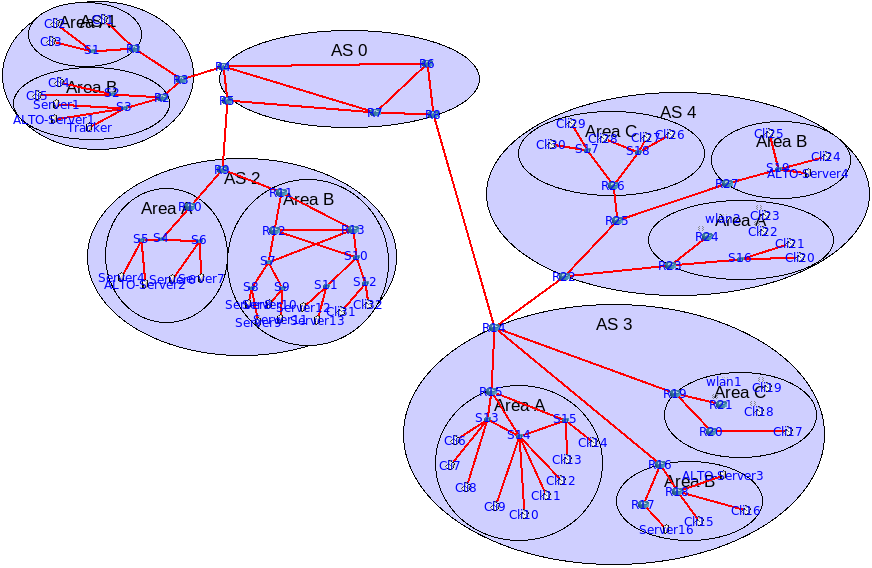
\includegraphics[scale=0.6]{img/topology-experiments-global}} \\
    \subfloat[View of AS0]{\label{exp-as0}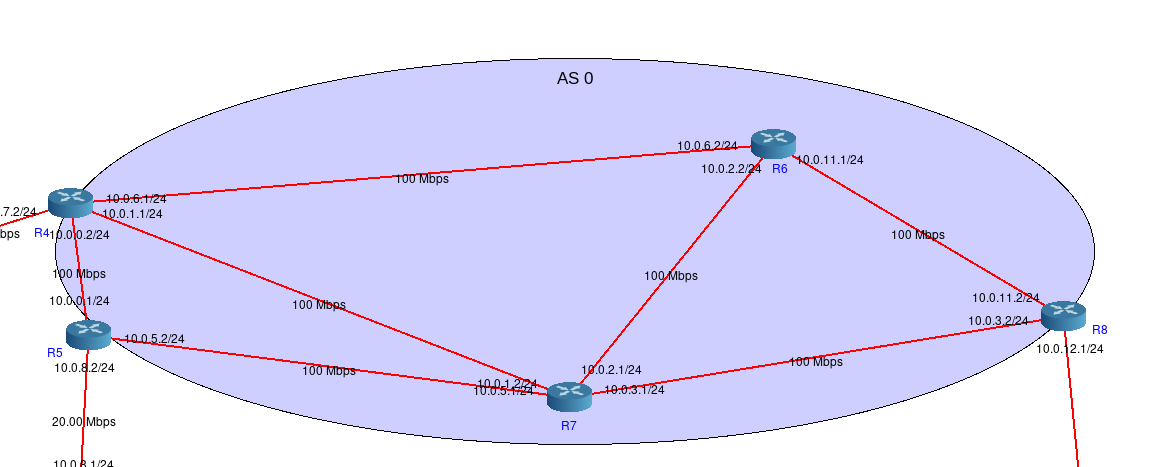
\includegraphics[scale=0.5]{img/topology-experiments-AS0}} \\
    \subfloat[View of AS1]{\label{exp-as1}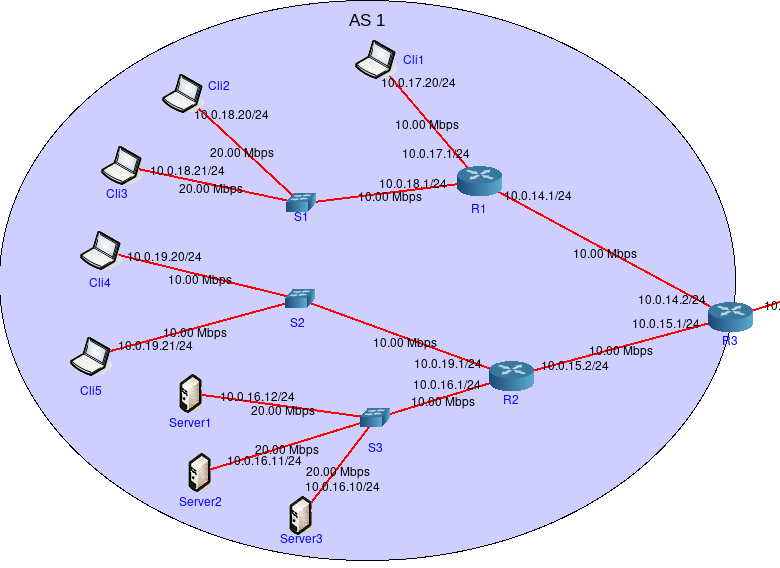
\includegraphics[scale=0.5]{img/topology-experiments-AS1}} \\
    \end{figure}

    \begin{figure}[H]\ContinuedFloat
    \centering
    \subfloat[View of AS2]{\label{exp-as2}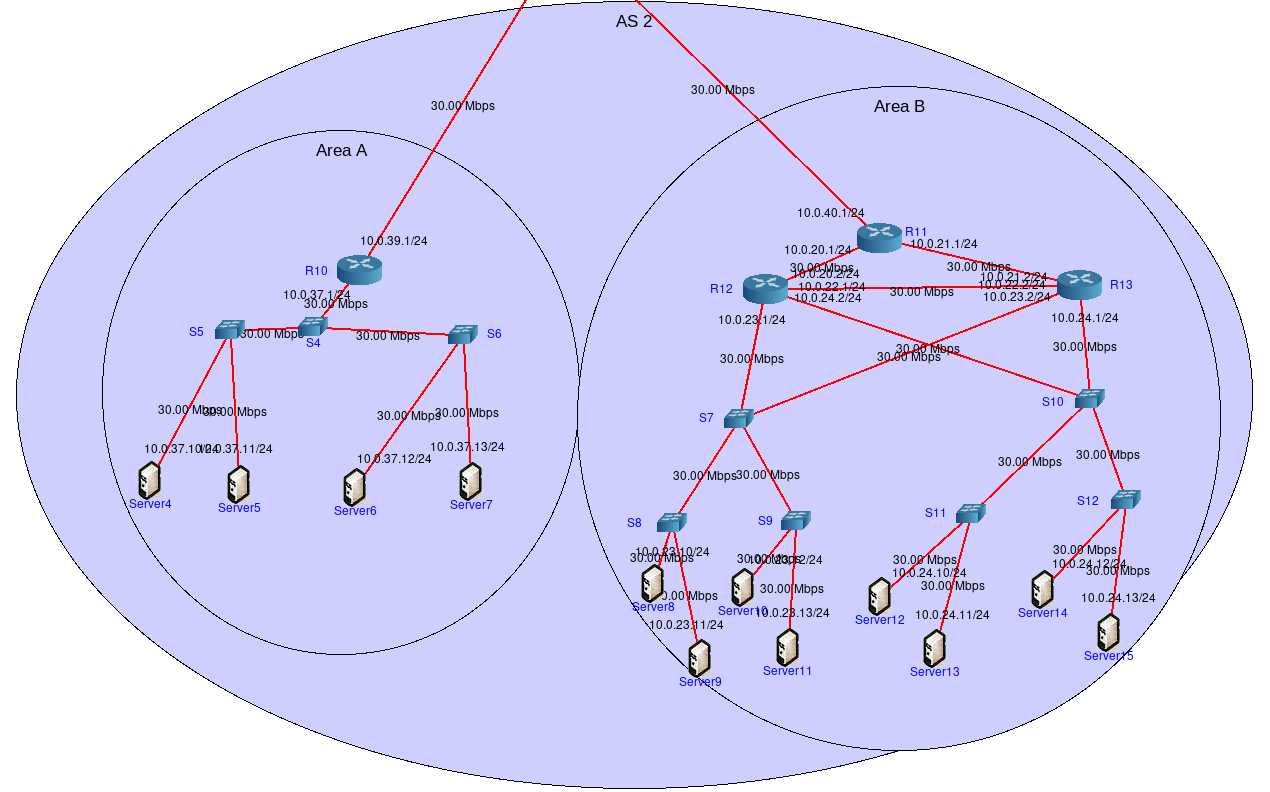
\includegraphics[scale=0.5]{img/topology-experiments-AS2}} \\
    \subfloat[View of AS3]{\label{exp-as3}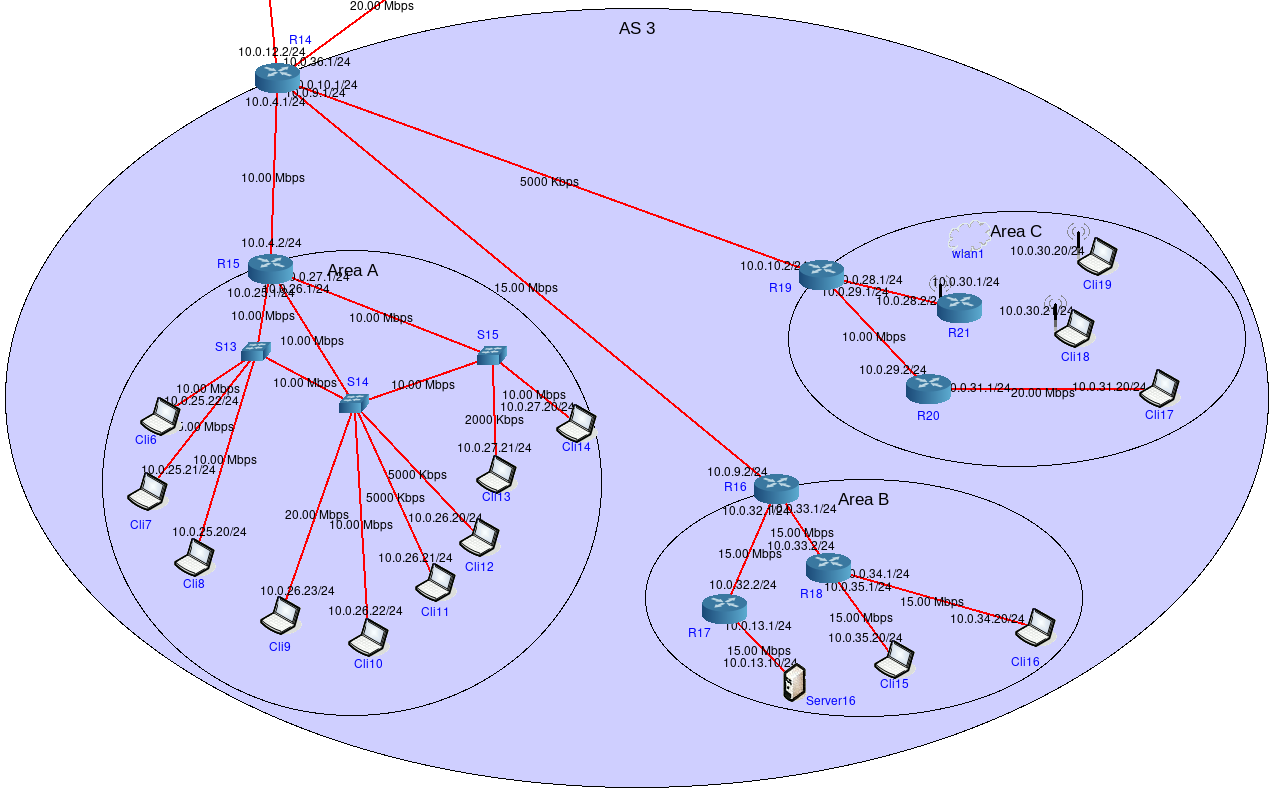
\includegraphics[scale=0.5]{img/topology-experiments-AS3}} \\
    \end{figure}

    \begin{figure}[H]\ContinuedFloat
    \centering
    \subfloat[View of AS4]{\label{exp-as4}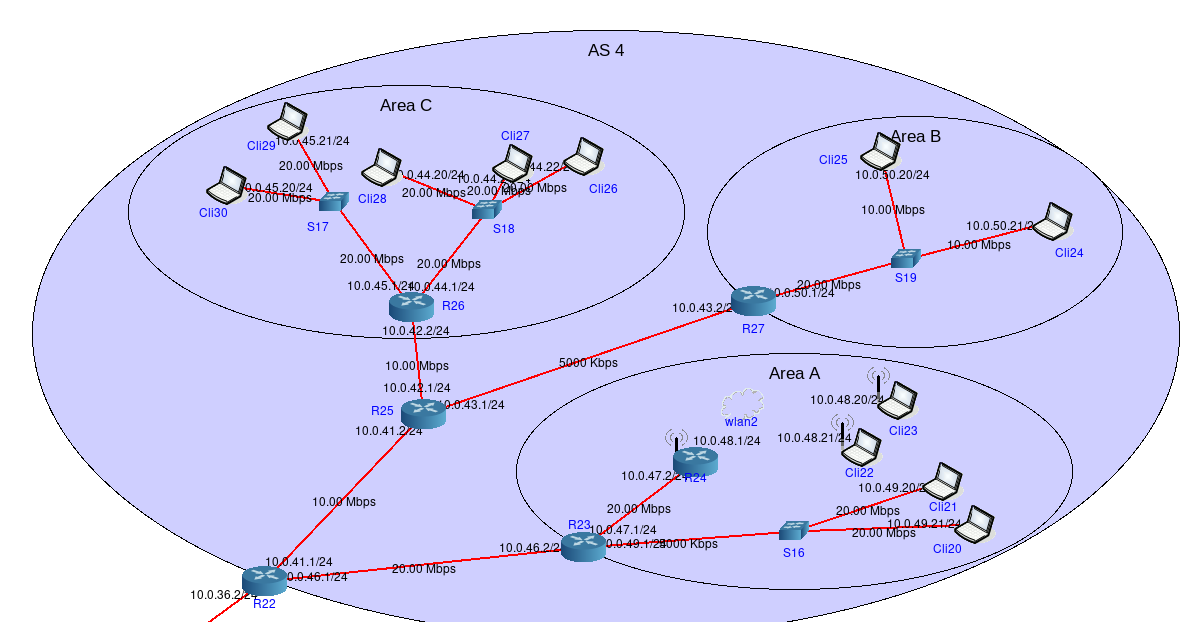
\includegraphics[scale=0.5]{img/topology-experiments-AS4}} \\
%    \caption{Global caption that can reference}
    \caption{values for different arms (cont.)}
    \label{fig:test-topology}
    \end{figure}

    Each node on the network has a given purpose that is represented as a node label, and link labels are used to specify connection properties.
    Unless stated otherwise with these labels, all other properties are equal throughout the network.
    Some pre-packaged \gls{core} services need to be enabled to assure network connectivity - mainly \gls{ospfv3} and \gls{bgp} - and scripting is used to, at the beginning of the simulation, bootstrap programs in specific nodes.
    This is done by utilizing the command line utility vcmd that runs specified commands in control channels that are created at runtime by \gls{core} - for example, the following command executes a ping command to address "10.0.0.1" with origins on node "P2P-Cli-1" and on simulation session 12345:

    \begin{center}
    \begin{lstlisting}[caption=Execution of an example command through the control channel of a given node, language=bash]
$ vcmd -c /tmp/pycore.12345/P2P-Client-1 -- ping 10.0.0.1
    \end{lstlisting}
    \end{center}

\section{Scenarios}

\subsection{Scenario 1 - P2P file sharing}

\textbf{Description:} All "CliN" nodes in the network, with N from 1 to N, actively serve all ten equally sized fragments of a 1GB file to other pers, and the bootstrapping method includes informing the tracker about what file fragments they serve.
    \ref{table:fragment-allocations} shows what endpoints possess what file fragment IDs.

\begin{table}[H]
\centering
\hspace*{-0.5em}
\begin{tabular}{|c|l|}
    \hline
    \textbf{Fragment ID} & \textbf{Available endpoints}                  \\ \hline
    x00                  & ["10.0.18.21", "10.0.24.20", "10.0.35.20"],   \\ \hline
    x01                  & ["10.0.18.20", "10.0.26.21", "10.0.48.21"],   \\ \hline
    x02                  & ["10.0.19.21", "10.0.24.21", "10.0.35.20"],   \\ \hline
    x03                  & ["10.0.24.21", "10.0.27.21", "10.0.31.20"],   \\ \hline
    x04                  & ["10.0.18.21", "10.0.26.23", "10.0.24.20"],   \\ \hline
    x05                  & ["10.0.19.20", "10.0.24.20", "10.0.24.21"],   \\ \hline
    x06                  & ["10.0.27.21", "10.0.48.20", "10.0.49.21"],   \\ \hline
    x07                  & ["10.0.48.21", "10.0.49.21", "10.0.50.21"],   \\ \hline
    x08                  & ["10.0.50.20", "10.0.50.21", "10.0.35.20"],   \\ \hline
    x09                  & ["10.0.25.22", "10.0.26.21", "10.0.31.20"]    \\ \hline
\end{tabular}
\caption{Tracker mappings of file fragments to available endpoints}
\label{table:fragment-allocations}
\end{table}

    "Cli2" wishes to retrieve that file, and to do so he firstly contacts "Tracker" for tracking information in the form of a file that contains a mapping between a fragment \gls{id} and the suggested peer, alongside with the file's checksum.
    After retrieveing the mapping, the client will sequencially request each fragment from its appointed peer, finalizing with the merge all the fragments into a single file and calculating the checksum that will be compared with the one provided by the tracker.
    An \gls{alto} server resides in the same \gls{as} and maintains resources - specifically, a local network map that groups peers within locality as within "Area A" of "AS1", "Area B" of "AS2", or externally to "AS1".
    It also maintains global resources - specifically, an endpoint cost map indicating expected bandwidth and delay between all the peers participating in the overlay \gls{p2p} network.

    \textbf{Variables:} The variable actions to be tested are how the tracker selects what candidate peer, from the pool of the available ones, will be selected to serve a given file fragment to the requesting peer.
    Table \ref{table:s1-tracker-methods} displays the different tracker algorithms that will be tested for the task of peer matching.

\begin{table}[H]
\centering
\hspace*{-0.5em}
\begin{tabular}{|l|L|}
    \hline
    \textbf{Tracker Algorithm} & \multicolumn{1}{m{11cm}|}{\textbf{Description}}                                                                         \\ \hline
    Random                     & \multicolumn{1}{m{11cm}|}{Randomly elect among all available peers}                                                     \\ \hline
    RTT                        & \multicolumn{1}{m{11cm}|}{Select the peer with the smallest probe packet \gls{rtt} measurement average in 10 pings}     \\ \hline
    ALTO - Local               & \multicolumn{1}{m{11cm}|}{Retrieve the local network map from the requesting peer's \gls{alto} server and discover the peers whose \gls{pid} matches the requesting peer, choosing randomly if multiple options exist}                                                                                                           \\ \hline
    ALTO - Global              & \multicolumn{1}{m{11cm}|}{Retrieve the global multicost endpoint cost map from the requesting peer's \gls{alto} server by selecting the tcp throughput and one way delay metrics, and selecting the peer that maximizes throughput with a delay no bigger than 5 milliseconds.}                                                  \\ \hline
\end{tabular}
\caption{Tracker algorithms to be tested in scenario 1}
\label{table:s1-tracker-methods}
\end{table}

\textbf{Measurements:} The measurements will target network resource usage and application performance.
Table \ref{table:s1-measurements} presents the measurements that will be collected during the experiment runs.

\begin{table}[H]
\centering
\hspace*{-1.2em}
\begin{tabular}{|l|l|L|}
    \hline
    \textbf{Measurement}     & \textbf{Units}     & \multicolumn{1}{m{10cm}|}{\textbf{Description}}  \\ \hline
    Transfer Time            & Seconds            & \multicolumn{1}{m{10cm}|}{Total amount of time required to transfer all file fragments} \\ \hline
    Network Traffic          & Megabytes          & \multicolumn{1}{m{10cm}|}{Total amount of traffic that entered each network area and AS} \\ \hline
\end{tabular}
\caption{Measurements to be taken in scenario 1}
\label{table:s1-measurements}
\end{table}


\subsubsection{Scenario 2 - HTTP transfer scheduling}

    \textbf{Description:} "Server1" in "AS1" acts as a server of \gls{http} content.
    "Cli1" wishes to retrieve a 500MB file from that server in one single session.
    The server is subjected to variable, random client loads that affect processing and storage power, and subsequently its ability to serve clients, as well as periodic traffic loads within the \gls{as} whenever the server clusters in that system enchange data between themselves for server redundancy and general synchronization.
    This will be translated in practice as dynamically variable round-trip delay from "Cli1" to "Server1", which is specifically shown in \ref{table:server-delays}

\begin{table}[H]
\centering
\begin{tabular}{|l|c|}
    \hline
    \textbf{Simulation time}  & \textbf{Client-Server path delay}  \\ \hline
    0 seconds                 & 100 ms                             \\ \hline
    60 seconds                & 50 ms                              \\ \hline
    120 seconds               & 20 ms                              \\ \hline
    180 seconds - \infty      & 10 ms                              \\ \hline
\end{tabular}
\caption{Dynamically applied client-server path delays}
\label{table:server-delays}
\end{table}


    The data center administrator mantains a cost map calendar where he registers all reserved backup transfers with two purposes: to keep track of all scheduled transfers so further ones can be scheduled as not to clash with pre-reserved ones, and to signal to \gls{alto} clients when \gls{qos} levels to those servers are expected to degrade.

\textbf{Variables: } The variable action to be tested is how the \gls{http} client selects the most appropriate time to retrieve the content from the server.
Table \ref{table:s2-client-methods} displays the different client algorithms that will be tested for the task of server request scheduling.

\begin{table}[H]
\begin{tabular}{|l|L|}
    \hline
    \textbf{Client Algorithm} & \multicolumn{1}{m{11cm}|}{\textbf{Description}}                                                                     \\ \hline
    Immediate                 & \multicolumn{1}{m{11cm}|}{Immediatelly request the resource from the server}                                        \\ \hline
    RTT                       & \multicolumn{1}{m{11cm}|}{Ping the server every 5 seconds and request the resource when the delay is below 20ms}                                                                                                                                                                          \\ \hline
    ALTO                      & \multicolumn{1}{m{11cm}|}{Retrieve a calendar cost map from the \gls{alto} server in AS2 of expected path delay to the server, and iniciate immediately when the delay is expected to drop below 20ms}                                                                                    \\ \hline
\end{tabular}
\caption{Client algorithms to be tested in scenario 2}
\label{table:s2-client-methods}
\end{table}

\textbf{Measurements:} Table \ref{table:s2-measurements} presents the measurements that will be collected during the experiment runs.

\begin{table}[H]
\centering
\begin{tabular}{|l|l|L|}
    \hline
    \textbf{Measurement}        & \textbf{Units}     & \multicolumn{1}{m{7cm}|}{\textbf{Description}}                                                  \\ \hline
    Transfer Time               & Seconds            & \multicolumn{1}{m{7cm}|}{Total amount of time required to transfer the file}                    \\ \hline
    Network Traffic             & Megabytes          & \multicolumn{1}{m{7cm}|}{Total amount of traffic that passed through each area network and AS}  \\ \hline
\end{tabular}
\caption{Measurements to be taken in scenario 2}
\label{table:s2-measurements}
\end{table}

\subsection{Scenario 3 - HTTP mirror selection}

\textbf{Description:} An \gls{http} client wishes to retrieve a 500MB file from a server.
After querying the public proxy, an index is provided which contains a address lists of the four mirror servers that provide that content.
The listing is show in table \ref{table:server-mirrors}

\begin{table}[H]
\centering
\begin{tabular}{|l|c|c|}
    \hline
    \textbf{Server address} & \textbf{AS} & \textbf{Area} \\ \hline
    10.0.16.12              & 1           & B             \\ \hline
    10.0.37.10              & 2           & A             \\ \hline
    10.0.23.11              & 2           & B             \\ \hline
    10.0.13.10              & 3           & B             \\ \hline
\end{tabular}
\caption{Listed server mirrors}
\label{tabel:server-mirrors}
\end{table}

The mirror servers will be subjected to constant loads at the start of the scenario, that are translated as throughput throttling applied from the client to the servers, specifically the ones shown in \ref{table:mirrors-bandwidth}.

\begin{table}[H]
\centering
\begin{tabular}{|l|c|}
    \hline
    \textbf{Server address} & \textbf{Throughput} \\ \hline
    10.0.16.12              & 3.0  ms             \\ \hline
    10.0.37.10              & 5.0  ms             \\ \hline
    10.0.23.11              & 10.0 ms             \\ \hline
    10.0.13.10              & 5.0  ms             \\ \hline
\end{tabular}
\caption{Listed server mirrors}
\label{tabel:server-mirrors}
\end{table}

The \gls{alto} server local to that client provides a global \gls{alto} endpoint property map that contains \gls{cpu} and \gls{ram} load information about all the mirrors, as well as an endpoint cost map containing information about the expected bandwidth and delay from the client to the mirror.

\textbf{Variables: } The variable action to be tested is how the \gls{http} client selects which mirror server to retrieve the file from.
Table \ref{table:s3-client-methods} displays the different client algorithms that will be tested for the task of mirror selection.

\begin{table}[H]
\centering
\begin{tabular}{|l|L|}
    \hline
    \textbf{Client Algorithm} & \multicolumn{1}{m{11cm}|}{\textbf{Description}}                                                                                                               \\ \hline
    Random                    & \multicolumn{1}{m{11cm}|}{Randomly select a server }                                                                                                          \\ \hline
    Bandwidth                 & \multicolumn{1}{m{11cm}|}{Probe for available TCP throughput to the mirrors, and select the one with most bandwidth}   \\ \hline
    ALTO                      & \multicolumn{1}{m{11cm}|}{Retrieve an endpoint property map and endpoint cost map from the local \gls{alto} server, and choose the with most available bandwidth and delay below 2ms, whose memory and processing power is below 30\%} \\ \hline
\end{tabular}
\caption{Client algorithms to be tested in scenario 3}
\label{table:s2-client-methods}
\end{table}

\textbf{Measurements:} Table \ref{table:s3-measurements} presents the measurements that will be collected during the experiment runs.

\begin{table}[H]
\centering
\begin{tabular}{|l|l|L|}
    \hline
    \textbf{Measurement}        & \textbf{Units}     & \multicolumn{1}{m{7cm}|}{\textbf{Description}}                                                  \\ \hline
    Transfer Time               & Seconds            & \multicolumn{1}{m{7cm}|}{Total amount of time required to transfer the file}                    \\ \hline
    Network Traffic             & Megabytes          & \multicolumn{1}{m{7cm}|}{Total amount of traffic that passed through each area network and AS}  \\ \hline
\end{tabular}
\caption{Measurements to be taken in scenario 3}
\label{table:s2-measurements}
\end{table}

\section{Results}

This section will show the observed results for each of the simulated scenarios, highlighting how the different variable methods compared to each other.

\subsection{Scenario 1}

Figure \ref{fig:graph-execution-scenario1} shows the obtained execution times for each of the variable methods in scenario 1.
It appears that the method of probing for path delay was the worst, at 1096 seconds of runtime, closely followed by the method of randomly selecting between the available peers.
Considerably faster are the \gls{alto}-related options.
The one considering a local server with its own information aided the application in achieving a 913.19 seconds execution time, whereas a global approach was able to considerably shave more time, at around 821.92 total seconds.

\begin{figure}[H]
\centering
\begin{tikzpicture}
    \begin{axis}[ 
        xbar,xmin=0,xmax=1500,
        xlabel={Execution times (s)},
        symbolic y coords={{ALTO-Global},{ALTO-Local},{RTT},{Random}},
        xtick={0, 500, 1000, 1500},
        ytick=data,
        nodes near coords, nodes near coords align={horizontal},
        ytick=data,
    ]
    \addplot[fill=lightblue] coordinates {(1096.314,{RTT}) (913.194,{ALTO-Local}) (821.915,{ALTO-Global}) (1052.820,{Random})};
    \end{axis}
\end{tikzpicture} %width=6cm,height=7.59cm
\caption{Execution times measured Scenario 1}
\label{fig:graph-execution-scenario1}
\end{figure}

Figure \ref{fig:graph-traffic-scenario1} show the measured traffic influx into the network's \glspl{as} and their areas.
It can be immediatelly identified that the delay probing method incurred in considerable amount of traffic entering the local \gls{as} from the exterior.
A random approach reduced that value almost in half, but the \gls{alto} approaches were both equally proficient and had the lowest amount of incoming exterior traffic.
The rest of the measurements was negligible in how tiny they were, with small bumps in "AS3" indicating choice preference for the delay-measuring method.
 
\begin{figure}[H]
\centering
\begin{tikzpicture}
    \pgfplotsset{%
        width=10cm,
        height=24cm
    }
    \begin{axis}[
        xbar,xmin=0,xmax=2500,
        bar width=8,
        xlabel={Traffic influx by region (bytes)},
        symbolic y coords={{ALTO-Global},{ALTO-Local},{RTT},{Random}},
        xtick={0, 500, 1000, 1500, 2000, 2500},
        enlarge y limits  = 0.2,
        enlarge x limits  = 0.01,
        typeset ticklabels with strut,
        legend pos=outer north east,
        ytick=data,
        nodes near coords, nodes near coords align={horizontal},
        ytick=data,
        reverse legend,
        legend image code/.code={
        \draw [#1] (0cm,-0.1cm) rectangle (0.5cm,0.1cm); }
    ]

    % Area 4 - Area C
    \addplot[fill=ao(english)] coordinates {(1.55280,{RTT}) (0.078516,{ALTO-Local}) (0.074514,{ALTO-Global}) (0.155280,{Random})};

    % Area 4 - Area B
    \addplot[fill=armygreen] coordinates {(2.817773,{RTT}) (0.077420,{ALTO-Local}) (0.074318,{ALTO-Global}) (2.817773,{Random})};

    % Area 4 - Area A
    \addplot[fill=applegreen] coordinates {(10.104310,{RTT}) (5.181086,{ALTO-Local}) (2.559743,{ALTO-Global}) (10.104310,{Random})};

    % AS 4
    \addplot[fill=green] coordinates {(12.763713,{RTT}) (5.177578,{ALTO-Local}) (2.556691,{ALTO-Global}) (5.058152,{Random})};

    % AS 3 - Area C
    \addplot[fill=canaryyellow] coordinates {(5.476332,{RTT}) (2.737291,{ALTO-Local}) (0.072710,{ALTO-Global}) (5.476332,{Random})};

    % AS 3 - Area B
    \addplot[fill=aureolin] coordinates {(5.424188,{RTT}) (0.077640,{ALTO-Local}) (2.707887,{ALTO-Global}) (5.424188,{Random})};

    % AS 3 - Area A
    \addplot[fill=bananayellow] coordinates {(5.133640,{RTT}) (2.562905,{ALTO-Local}) (5.045584,{ALTO-Global}) (5.133640,{Random})};

    % AS 3
    \addplot[fill=amber] coordinates {(28.322497,{RTT}) (10.322792,{ALTO-Local}) (10.159846,{ALTO-Global}) (12.840053,{Random})};

    % AS2 - Area B
    \addplot[fill=awesome] coordinates {(10.699966,{RTT}) (2.711305,{ALTO-Local}) (2.707281,{ALTO-Global}) (10.699966,{Random})};

    % AS2 - Area A
    \addplot[fill=alizarin] coordinates {(0.157304,{RTT}) (0.079984,{ALTO-Local}) (0.076102,{ALTO-Global}) (0.157304,{Random})};

    % AS2 
    \addplot[fill=red] coordinates {(10.697794,{RTT}) (2.709763,{ALTO-Local}) (2.707499,{ALTO-Global}) (7.993195,{Random})};

    % AS1 - Area B
    \addplot[fill=navy-blue] coordinates {(0.160326,{RTT}) (5.052812,{ALTO-Local}) (5.047120,{ALTO-Global}) (0.088108,{Random})};
    % AS1 - Area A
    \addplot[fill=lightblue] coordinates {(1710.524046,{RTT}) (798.246822,{ALTO-Local}) (798.246910,{ALTO-Global}) (912.287378,{Random})};
    % AS1
    \addplot[fill=blue] coordinates {(1711.189266,{RTT}) (570.387434,{ALTO-Local}) (570.421828,{ALTO-Global}) (912.733470,{Random})};

    \legend{AS4-AreaC, AS4-AreaB, AS4-AreaA, AS4, AS3-AreaC, AS3-AreaB, AS3-AreaA, AS3, AS2-AreaB, AS2-AreaA, AS2, AS1-AreaB, AS1-AreaA, AS1}
    \end{axis}
\end{tikzpicture}
\caption{Inbound traffic flux by network areas measured in Scenario 1}
\label{fig:graph-traffic-scenario1}
\end{figure}

\subsection{Scenario 2}

Figure \ref{fig:graph-execution-scenario2} shows the obtained execution times for each of the variable methods in scenario 2.
It appears that the \gls{alto}-aided and delay-probing methods were equally circling a 640 second runtime, and an approach of immediately querying the server was faster, at 457.19 seconds.

\begin{figure}[H]
\centering
\begin{tikzpicture}
    \begin{axis}[ 
        xbar,xmin=0,xmax=1500,
        xlabel={Execution times (s)},
        symbolic y coords={{ALTO-Global},{RTT},{Immediate}},
        xtick={0, 500, 1000, 1500},
        ytick=data,
        nodes near coords, nodes near coords align={horizontal},
        ytick=data,
    ]
    \addplot[fill=lightblue] coordinates {(641.998,{RTT}) (457.186,{Immediate}) (636.456,{ALTO-Global})};
    \end{axis}
\end{tikzpicture} %width=6cm,height=7.59cm
\caption{Execution times measured Scenario 2}
\label{fig:graph-execution-scenario2}
\end{figure}

Figure \ref{fig:graph-traffic-scenario2} shows the measured traffic influx into the network's \glspl{as} and their areas.
Disregarding negligible measurements from given \glspl{as} and areas, it appears that the method utilizing ping measurements had slight, but existing, increased traffic that had its influx on AS1's areas. 

\begin{figure}[H]
\centering
\begin{tikzpicture}
    \pgfplotsset{%
        width=10cm,
        height=24cm
    }
    \begin{axis}[
        xbar,xmin=0,xmax=700,
        xlabel={Traffic influx by region (bytes)},
        symbolic y coords={{ALTO-Global},{RTT},{Immediate}},
        xtick={0, 100, 200, 300, 400, 500, 600, 650, 700},
        enlarge y limits  = 0.2,
        enlarge x limits  = 0.01,
        typeset ticklabels with strut,
        legend pos=outer north east,
        ytick=data,
        nodes near coords, nodes near coords align={horizontal},
        ytick=data,
        reverse legend,
        legend image code/.code={
        \draw [#1] (0cm,-0.1cm) rectangle (0.5cm,0.1cm); }
    ]

    % Area 4 - Area C
    \addplot[fill=ao(english)] coordinates {(0.062080,{RTT}) (0.064590,{ALTO-Global}) (0.052496,{Immediate})};

    % Area 4 - Area B
    \addplot[fill=armygreen] coordinates {(0.062202,{RTT}) (0.064378,{ALTO-Global}) (0.052198,{Immediate})};

    % Area 4 - Area A
    \addplot[fill=applegreen] coordinates {(0.062950,{RTT}) (0.063576,{ALTO-Global}) (0.052334,{Immediate})};

    % AS 4
    \addplot[fill=green] coordinates {(0.061240,{RTT}) (0.061170,{ALTO-Global}) (0.052298,{Immediate})};

    % AS 3 - Area C 
    \addplot[fill=canaryyellow] coordinates {(0.062496,{RTT}) (0.062794,{ALTO-Global}) (0.053866,{Immediate})};
    % AS 3 - Area B 
    \addplot[fill=aureolin] coordinates {(0.064296,{RTT}) (0.063370,{ALTO-Global}) (0.055118,{Immediate})};
    % AS 3 - Area A 
    \addplot[fill=bananayellow] coordinates {(0.065532,{RTT}) (0.065106,{ALTO-Global}) (0.054766,{Immediate})};

    % AS 3
    \addplot[fill=amber] coordinates {(0.061992,{RTT}) (0.059772,{ALTO-Global}) (0.050814,{Immediate})};

    % AS2 - Area B
    \addplot[fill=awesome] coordinates {(0.064102,{RTT}) (0.064378,{ALTO-Global}) (0.056352,{Immediate})};

    % AS2 - Area A
    \addplot[fill=alizarin] coordinates {(0.064144,{RTT}) (0.065730,{ALTO-Global}) (0.054380,{Immediate})};

    % AS2 
    \addplot[fill=red] coordinates {(0.062908,{RTT}) (0.059772,{ALTO-Global}) (0.054064,{Immediate})};

    % AS1 - Area B
    \addplot[fill=navyblue] coordinates {(12.495609,{RTT}) (12.465589,{ALTO-Global}) (12.405077,{Immediate})};
    % AS1 - Area A
    \addplot[fill=lightblue] coordinates {(570.188334,{RTT}) (570.188204,{ALTO-Global}) (570.231908,{Immediate})};
    % AS1
    \addplot[fill=blue] coordinates {(0.066468,{RTT}) (0.066322,{ALTO-Global}) (0.059374,{Immediate})};

    \legend{AS4-AreaC, AS4-AreaB, AS4-AreaA, AS4, AS3-AreaC, AS3-AreaB, AS3-AreaA, AS3, AS2-AreaB, AS2-AreaA, AS2, AS1-AreaB, AS1-AreaA, AS1}
    \end{axis}
\end{tikzpicture}
\caption{Inbound traffic flux by network areas measured in Scenario 2}
\label{fig:graph-traffic-scenario2}
\end{figure}

\subsection{Scenario 3}

Figure \ref{fig:graph-execution-scenario3} shows the obtained execution times for each of the variable methods in scenario 3.
An approach of randomly choosing mirror servers had the worst performance time wise, with 912.39 seconds, and the \gls{tcp} throughput measuring method following with 496.57 seconds.
Finally, the \gls{alto}-aided approach was the quickest with 456.21 seconds of runtime.

\begin{figure}[H]
\centering
\begin{tikzpicture}
    \begin{axis}[ 
        xbar,xmin=0,xmax=1200,
        xlabel={Execution times (s)},
        symbolic y coords={{ALTO-Global},{Bandwidth},{Random}},
        xtick={0, 500, 1000, 1200},
        ytick=data,
        nodes near coords, nodes near coords align={horizontal},
        ytick=data,
    ]
    \addplot[fill=lightblue] coordinates {(456.212,{ALTO-Global}) (496.567,{Bandwidth}) (912.394,{Random})};
    \end{axis}
\end{tikzpicture} %width=6cm,height=7.59cm
\caption{Execution times measured Scenario 3}
\label{fig:graph-execution-scenario3}
\end{figure}

Figure \ref{fig:graph-traffic-scenario3} shows the measured traffic influx into the network's \glspl{as} and their areas.
It appears that the approach that probed for path bandwidth had a considerable impacts on the generated traffic influx, and the spikes of traffic in the random and \gls{alto} approach give clues into the selected mirrors - those residing in AS3-B and AS2-B, most specifically.

\begin{figure}[H]
\centering
\begin{tikzpicture}
    \pgfplotsset{%
        width=10cm,
        height=24cm
    }
    \begin{axis}[
        xbar,xmin=0,xmax=700,
        enlarge y limits  = 0.2,
        enlarge x limits  = 0.01,
        xlabel={Traffic influx by region (bytes)},
        symbolic y coords={{ALTO-Global},{Bandwidth},{Random}},
        xtick={0, 100, 200, 300, 400, 500, 600, 650, 700},
        typeset ticklabels with strut,
        legend pos=outer north east,
        nodes near coords, nodes near coords align={horizontal},
        ytick=data,
        reverse legend,
        legend image code/.code={
        \draw [#1] (0cm,-0.1cm) rectangle (0.5cm,0.1cm); }
    ]
    % AS 4 - Area C
    \addplot[fill=ao(english)] coordinates {(0.075912,{Random}) (0.055872,{Bandwidth}) (0.053384,{ALTO-Global})};

    % AS 4 - Area B
    \addplot[fill=armygreen] coordinates {(0.076426,{Random}) (0.055142,{Bandwidth}) (0.053358,{ALTO-Global})};

    % AS 4 - Area A
    \addplot[fill=applegreen] coordinates {(0.076176,{Random}) (0.054574,{Bandwidth}) (0.053664,{ALTO-Global})};

    % AS 4
    \addplot[fill=green] coordinates {(0.074608,{Random}) (0.054080,{Bandwidth}) (0.052362,{ALTO-Global})};

    % AS3 - Area C
    \addplot[fill=canaryyellow] coordinates {(0.077134,{Random}) (0.055872,{Bandwidth}) (0.054750,{ALTO-Global})};

    % AS3 - Area B
    \addplot[fill=aureolin] coordinates {(13.350893,{Random}) (0.055142,{Bandwidth}) (0.054312,{ALTO-Global})};

    % AS3 - Area A
    \addplot[fill=bananayellow] coordinates {(0.079726,{Random}) (0.058132,{Bandwidth}) (0.054394,{ALTO-Global})};

    % AS 3
    \addplot[fill=amber] coordinates {(13.348379,{Random}) (6.415429,{Bandwidth}) (0.051206,{ALTO-Global})};

    % AS2 - Area B
    \addplot[fill=awesome] coordinates {(0.078224,{Random}) (12.585748,{Bandwidth}) (13.202365,{ALTO-Global})};

    % AS2 - Area A
    \addplot[fill=alizarin] coordinates {(0.078416,{Random}) (25.785258,{Bandwidth}) (0.055618,{ALTO-Global})};

    % AS2 
    \addplot[fill=red] coordinates {(0.077014,{Random}) (38.313674,{Bandwidth}) (13.200761,{ALTO-Global})};

    % AS1 - Area B
    \addplot[fill=navyblue] coordinates {(0.080092,{Random}) (12.585188,{Bandwidth}) (0.056120,{ALTO-Global})};
    % AS1 - Area A
    \addplot[fill=lightblue] coordinates {(570.197962,{Random}) (571.161868,{Bandwidth}) (570.178424,{ALTO-Global})};
    % AS1
    \addplot[fill=blue] coordinates {(570.196112,{Random}) (571.481703,{Bandwidth}) (570.709008,{ALTO-Global})};

    \legend{AS4-AreaC, AS4-AreaB, AS4-AreaA, AS4, AS3-AreaC, AS3-AreaB, AS3-AreaA, AS3, AS2-AreaB, AS2-AreaA, AS2, AS1-AreaB, AS1-AreaA, AS1}
    \end{axis}
\end{tikzpicture}
\caption{Inbound traffic flux by network areas measured in Scenario 3}
\label{fig:graph-traffic-scenario3}
\end{figure}

\section{Discussion}
    \textbf{[Notes: The P2P client has no reasonable way to, without ISP cooperation, know that peers reside within network locality. A cited study used RTT heuristics that assumed that high RTT values exist in inter-ISP links, which may not always be the case. Randomly selecting is poor at optimal choice, but at the very least has potential for load balancing, something that the tracker itself can attempt to do on a per-locality basis, joining a best of both worlds. Leveraging only a network map to communicate peer locality is quick and takes little memory, and further experiments will add cost maps on top of it to mix both locality standards and QoS needs.]}

\todo{Finish discussion}

